\chapter{Flujos de Usuario}
\label{cp:user-flows}

\parindent0pt

En este trabajo, se definieron y documentaron los flujos de usuario para cada tipo de usuario identificado en el sistema durante la etapa de diseño de solución. Estos flujos de usuario permiten comprender cómo interactúan los diferentes actores con la plataforma con el objetivo de garantizar una experiencia de usuario intuitiva y eficiente antes de la ejecución de las pruebas de aceptación. A continuación, se describen los flujos de usuario para cada rol identificado: Productor Primario, Productor Secundario, Consumidor y Reciclador. Estos flujos fueron construidos a partir de los requerimientos funcionales definidos en la etapa de modelado y representan las principales interacciones de los distintos actores del sistema con la plataforma.

Inicialmente, todos los usuarios deben registrarse en la plataforma proporcionando información básica como correo electrónico y contraseña (Figura \ref{fig:flow-auth}). Al momento del registro, se debe elegir un rol para el usuario y, una vez creado, el usuario puede iniciar sesión para acceder a las funcionalidades correspondientes a su rol. Dentro de la plataforma, cada usuario puede acceder a la información de su perfil, pudiendo agregar el nombre de su empresa, su nombre y número de contacto (Figura \ref{fig:flow-user}). Adicionalmente, también disponen de la opción para cerrar sesión en cualquier momento.

Para los Productores Primarios (Figura \ref{fig:flow-primary-producer}), el flujo de uso incluye la posibilidad de registrar nuevos lotes de producción de envases, así como consultar el estado de los lotes existentes y consultar su trazabilidad. A su vez, estos usuarios pueden ver el inventario de material reciclable adquirido por la empresa para su reutilización en la producción.

En el caso de los Productores Secundarios (Figura \ref{fig:flow-secondary-producer}), el flujo de uso se centra en la gestión de los envases adquiridos. Estos usuarios pueden asignar sus envases a códigos de productos específicos, posibilitando así su trazabilidad posterior. A su vez, pueden consultar el estado de los envases adquiridos y su trazabilidad. Por último, pueden registrar sus ventas y controlar el stock de envases disponibles.

Los Consumidores (Figura \ref{fig:flow-consumer}), por su parte, pueden consultar información del origen de cualquier envase a partir de su código de producto. Pueden acceder a información detallada sobre los productos que han adquirido, incluyendo detalles sobre su trazabilidad y el ciclo de vida de los envases. Además, pueden reportar la entrega de envases a recicladores, pudiendo luego consultar el estado de cada uno de los envases reportados.

Finalmente, los Recicladores (Figura \ref{fig:flow-recycler}) pueden consultar el inventario de envases entregados por los consumidores, para clasificarlos y asignarlos a lotes de reciclaje según su composición. Estos usuarios pueden crear lotes de reciclaje y registrar la venta de material reciclado a productores primarios, cerrando así el ciclo de trazabilidad. A su vez, pueden consultar el origen de un envase recibido para reciclarlo correctamente.

A su vez, todos los usuarios pueden acceder a la funcionalidad de Seguimiento (Figura \ref{fig:flow-tracking}), donde pueden consultar el estado de cualquier envase registrado en la plataforma a partir de su código de producto o identificador. Esta funcionalidad permite a todos los actores del sistema verificar la trazabilidad y el ciclo de vida de los envases, promoviendo la transparencia y la confianza en el sistema.

\begin{figure}[!htb]
	\centering
	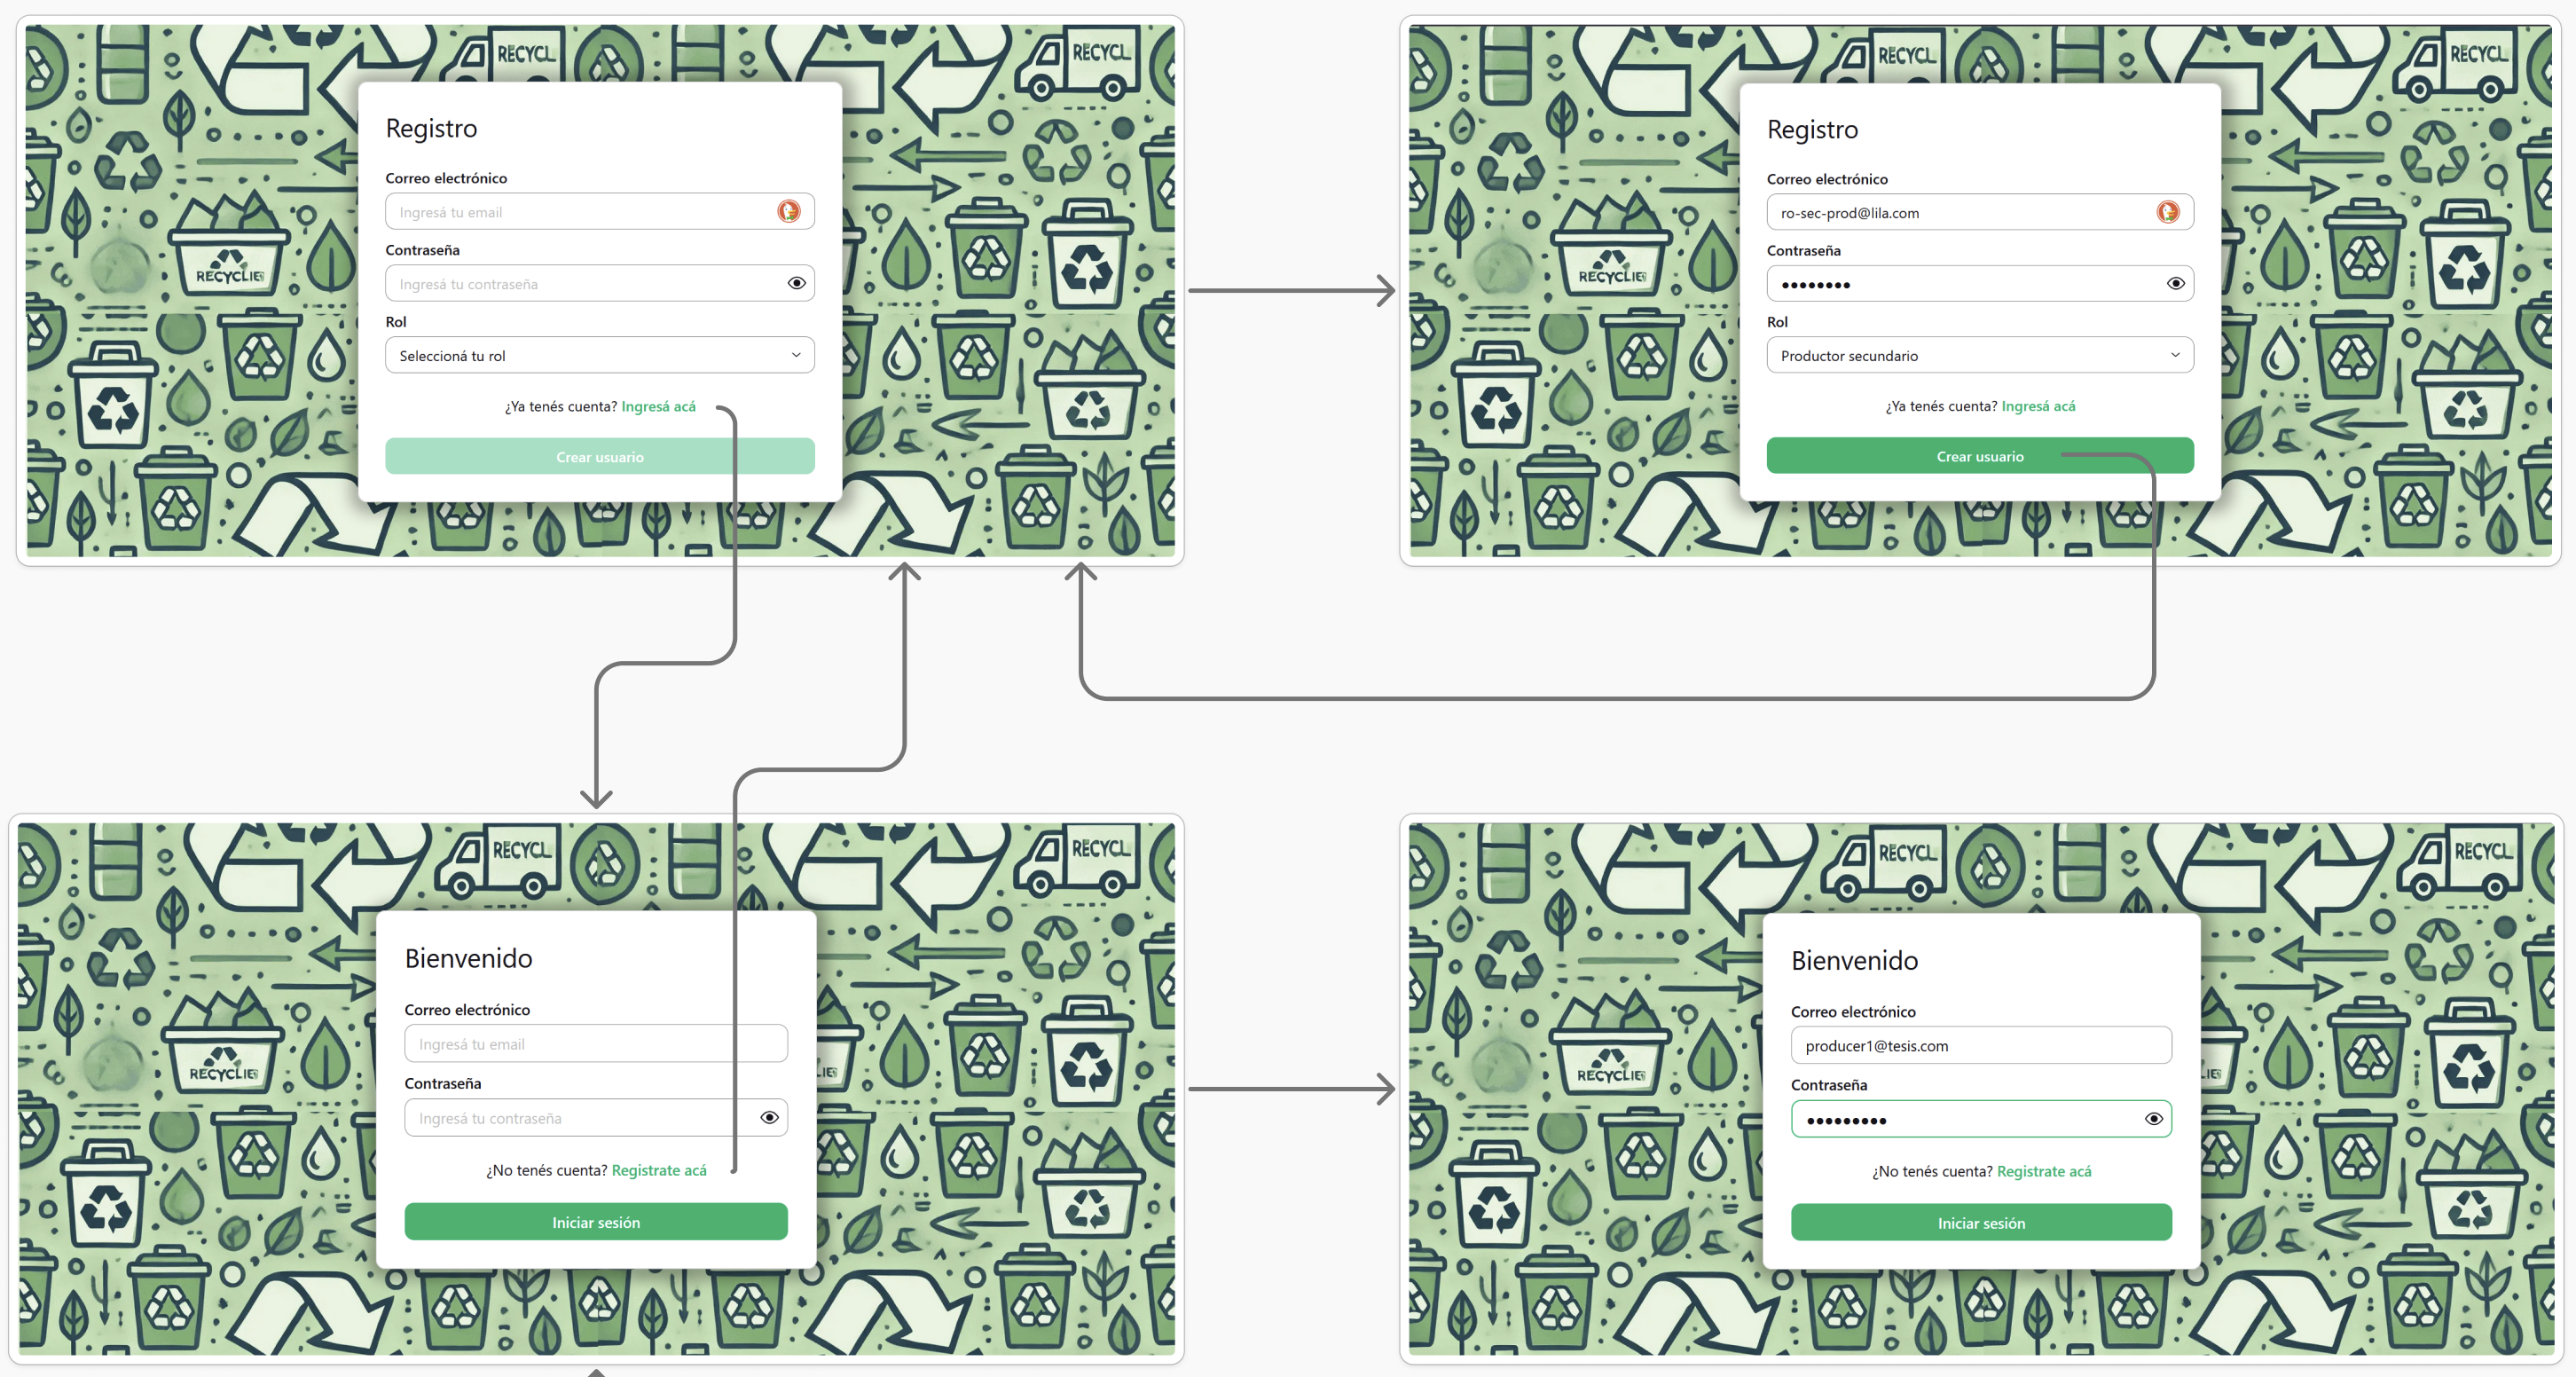
\includegraphics[width=\linewidth]{Figures/flow-auth.png}
	\caption{Flujo de autenticación de usuarios.}
  \label{fig:flow-auth}
\end{figure}

\begin{figure}[!htb]
	\centering
	\includegraphics[width=\linewidth]{Figures/flow-user.png}
	\caption{Flujo de gestión de usuarios.}
  \label{fig:flow-user}
\end{figure}

\begin{figure}[!htb]
	\centering
	\includegraphics[width=\linewidth]{Figures/flow-primary-producer.png}
	\caption{Flujo de productor primario.}
  \label{fig:flow-primary-producer}
\end{figure}

\begin{figure}[!htb]
	\centering
	\includegraphics[width=\linewidth]{Figures/flow-secondary-producer.png}
	\caption{Flujo de productor secundario.}
  \label{fig:flow-secondary-producer}
\end{figure}

\begin{figure}[!htb]
	\centering
	\includegraphics[width=\linewidth]{Figures/flow-consumer.png}
	\caption{Flujo de consumidor.}
  \label{fig:flow-consumer}
\end{figure}

\begin{figure}[!htb]
	\centering
	\includegraphics[width=\linewidth]{Figures/flow-recycler.png}
	\caption{Flujo de reciclador.}
  \label{fig:flow-recycler}
\end{figure}

\begin{figure}[!htb]
	\centering
	\includegraphics[width=\linewidth]{Figures/flow-tracking.png}
	\caption{Flujo de seguimiento de envases.}
  \label{fig:flow-tracking}
\end{figure}